\documentclass[12pt]{article}
\usepackage{geometry}                % See geometry.pdf to learn the layout options. There are lots.
\geometry{letterpaper}                   % ... or a4paper or a5paper or ... 
%\geometry{landscape}                % Activate for for rotated page geometry
\usepackage[parfill]{parskip}    % Activate to begin paragraphs with an empty line rather than an indent
\usepackage{./styles/daves,fancyhdr,natbib,graphicx,dcolumn,amsmath,lastpage,url}
\usepackage{amsmath,amssymb,epstopdf,longtable}
\usepackage[final]{pdfpages}
\DeclareGraphicsRule{.tif}{png}{.png}{`convert #1 `dirname #1`/`basename #1 .tif`.png}
\pagestyle{fancy}
\lhead{CE 5362 -- Surface WaterModeling}
\rhead{SPRING 2020}
\lfoot{}
\cfoot{}
\rfoot{Page \thepage\ of \pageref{LastPage}}
\renewcommand\headrulewidth{0pt}



\begin{document}
\begin{center}
{\textbf{{ CE 5362 Surface Water Modeling} \\ {Project 6}}}
\end{center}

\section*{{Introduction and Purpose}}
SToRM is a component of the USGS Multi-Dimensional Surface Water Modeling System \citep{mdswms2012}
SToRM is one of a generation of recently available 2--D hydrodynamic models available without charge or for low cost. 
This project is to gain experience using the model to determine if there is hydrodynamic evidence of circulation to explain potential erosion.


\section*{{Problem Background}}
A study of a portion of the White River at US 82 near Crosbyton, Texas.  
 The study site is located proximal to US 82 and within the Texas Department of Transportation Silver Falls Rest Area.  
 Figure \ref{fig:WhiteRiverAerial} is a Google Earth base image, with author drawn lines to indicate the approximate study area (brown lines), the thalweg (cyan), and four cross sectional elevation survey transects.   
Some additional elevations were also collected.  

\begin{figure}[h!] %  figure placement: here, top, bottom, or page
   \centering
   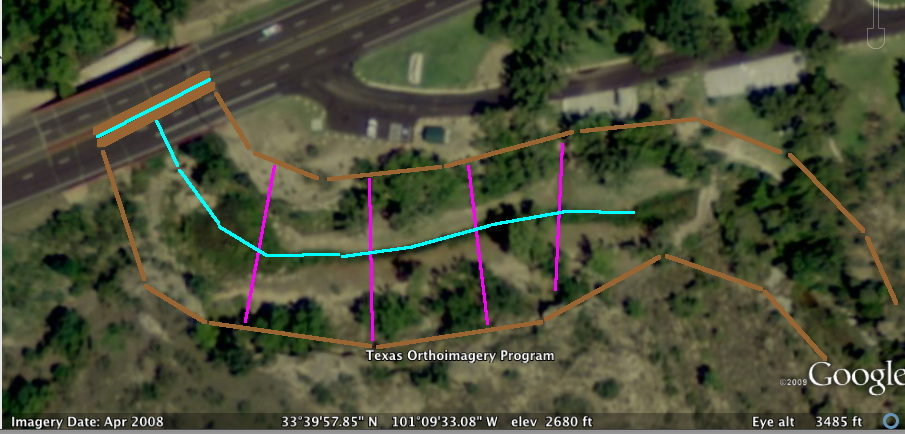
\includegraphics[width=6in]{WhiteRiverAerial.jpg} 
   \caption{Aerial view of White River case study.   Approximate location of thalweg, dam, and surveyed cross sections are indicated by the annotated segments.   Additional elevation locations are not depicted on the figure.  Flow is from left to right in this photograph.  Base image from \cite{GoogleEarth2011}.}
   \label{fig:WhiteRiverAerial}
\end{figure}
\clearpage

A dam is located near the west-bound bridge of US 82 (depicted in the photograph as the double thick brown lines).  
Remnants of tropical system ``Alex'' in early July, 2010 provided rain in the region and the peak rainfall near the site occurred on July 4, 2010.   
After this event, a USGS employee performed a post-storm field survey using conventional USGS slope-area computations to estimate the peak discharge at the site from the debris lines left by the discharge, and an independent estimate of flow over the Silver Falls dam.

\subsubsection*{Topographic Model for the White River}
SToRM uses a topographic database in XYZ format.   A Reflectorless Total Station was used to generate elevation survey data.
The elevations obtained by the cross sections survey of the White River site were converted into a topographic grid for input to SToRM using the kriging algorithm in Surfer \citep{surfer2010} to generate a topographic model for importing into SToRM.   A boundary polygon that roughly follows the brown outline in Figure \ref{fig:WhiteRiverAerial} was then applied to force a physical boundary into the model.    Figure \ref{fig:white-river-elevation-image} is a plot of the elevation survey coordinates and the gridded data.  
\begin{figure}[htbp] %  figure placement: here, top, bottom, or page
   \centering
   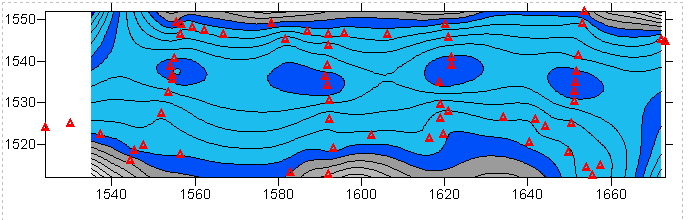
\includegraphics[width=6in]{white-river-elevation-image.jpg} 
   \caption{Contour map generated from gridded elevation survey.   
   Open triangles are locations of surveyed elevations in transformed XY coordinate system and are listed in
   file: \texttt{whiteriver-survey.tpo}. The contours are generated from the gridded values listed in file: \texttt{whiteriver-gridded.tpo} }
   \label{fig:white-river-elevation-image}
\end{figure}
  Analyst intervention was used in a grid-node editor to force certain elevations to be faithful to actual elevations observed in the two case studies. 
The two files for this project are \url{whiteriver-survey.tpo} and \url{whiteriver-gridded.tpo}.

Table \ref{tab:white-river-results} is a list of water surface elevations at the study site from the surveyed high water marks in the coordinate system of the two \url{.tpo} files

\begin{table}[ht!]
   \centering
      \caption{Measured Water Surface Elevations (in meters)}
   %\topcaption{Table captions are better up top} % requires the topcapt package
   \begin{tabular}{p{1in} p{1in} p{1in}  }
   Section & X Station (m)  & WSE$_{o} $(m)\\
   1 & 1554 & 27.52 \\
   2 & 1592 & 27.31 \\
   3 & 1618 & 27.04  \\
   4 & 1650 & 26.83  \\
   \end{tabular}
\label{tab:white-river-results}
\end{table}

\subsubsection*{Resistance Model}
Use a Manning's-type resistance model for frictional effect in SToRM because of simplicity in input; A Manning's n value of 0.04 is probably reasonable for the White River situation.
\subsubsection*{Boundary, Initial and Simulation Control Conditions}
The upstream boundary condition is a specified discharge ($1900~\frac{ft^3}{sec}$) that is to be distributed across a node string. 
The downstream boundary is a fixed stage.
The initial flow velocity should be set as the inlet discharge divided by the outlet cross sectional flow area (a  mean section velocity).  
The initial conditions in both simulations were to set the water surface at the same depth as the downstream boundary condition.   
A HEC-RAS model of the portion of White River can be used to estimate initial values for the SToRM model and is included in the problem data directory \url{whiteriver-hecras.zip}.
\section*{{Problem Statement}}
Build and run a SToRM model of the White River situation described above, write a brief report (like a lab report) and include:
\begin{enumerate}
\item Does there appear to be a circulation pattern in the 2D model?
\item Which topography file produces a better model (qualitative assessment, no computations are expected)? Explain your reasoning.
\item Does SToRM produce water surface elevations that are consistent with the HEC-RAS model?
\item Does SToRM produce water surface elevations consistent with observations ( X-station is given, choose a centerline location to compare for Y-station) ?
\item Produce vector plot of the flow pattern at $1900~\frac{ft^3}{sec}$ in the model
\item Produce streamline plot of the flow pattern at $1900~\frac{ft^3}{sec}$ in the model
\item Do the ``pits'' from the gridding algorithm seem to correlate with the flow patterns (qualitative assessment, no computations are expected), if so how?
\item (Advanced) Edit the \url{.tpo} file to move the cut to one side of the flume.  Does this change the velocity pattern.  Produce output plots.
\end{enumerate}


\begin{thebibliography}{}

\bibitem[USGS, 2011]{storm2011}
{USGS Geomorphology Laboratory} (2011).
\newblock System for Transport and River Modeling.   
\url{http://wwwbrr.cr.usgs.gov/projects/GEOMORPH_Lab/project-SToRM.html} Webpage last accessed, 12 Jan 2012.

\bibitem[McDonald and others, 2012]{mdswms2012}
{McDonald, R.R., Nelson, J.M., and Bennett, J.P.}, (2012).  
\textsl{in press}. Multi-dimensional surface-water modeling system user's guide: U.S. Geological Survey Techniques and Methods, 6-B2, 136 p.

\bibitem[Google Earth, 2011]{GoogleEarth2011}
{Google Earth, Google Inc.}, (2011). 
\url{http://www.google.com/earth/index.html} 
1600 Amphitheatre Parkway Mountain View, CA, 94043
%
\bibitem[Golden Software, 2010]{surfer2010}
{Golden Software, Inc.}, (2010). Surfer 10.
809 14th Street, Golden, Colorado 80401-1866, U.S.A.
Phone: 303-279-1021 Fax: 303-279-0909
\url{www.GoldenSoftware.com}

%\bibitem[Dixon, J. 2011]{dixon2011}
%{Dixon, J.}, (2011). 
%A Relation Between Select Hydraulic Properties and Sediment
%Transport Volume Through Experimental Culvert Configurations
%and Techniques for Measuring Sediment Transport Volumes.
%MS Thesis, Department of Civil and Environmental Engineering, Texas Tech University, 117 p.

\end{thebibliography}

\end{document}